\newpage
\section{Additional Information}
\label{sec:04_additionalInformation}

On top of the direction detection by \ac{TDOA}, additional information
can be won by received microphone data.
This information can be used to improve the single robot result or
to feed the team filter with beta information.
As \cref{subsec:03_distance} has described, the distance of the sound source
can be estimated approximately for nearby signals that are aligned with
the x-axis of the robot's head.
Another intuitive approach is the inspection of the \ac{SNR} which
is assumed as higher for closer sources.
Apart from this, the \ac{PSNR} of the \ac{GCC} defined in \cref{subsec:03_snr,subsec:03_psnr}
is investigated.

\subsection{Distance Approximation}
\label{subsec:04_distance}

\Cref{subsec:03_distance} clarified the conditions to identify the distance of
the sound source by one robot.
To examine the validity of this statement, measurements from the front and
back of the robot are collected and evaluated.
\Cref{tab:04_distance} lists the distances and their results by the
all methods.
For both measurements with zero distance, the orientation of the whistle differed.
180\si{\degree} indicates that the whistle was turned in the opposite direction
of the robot.
In the other case (0\si{\degree}), the whistle was aligned with the robot.
The distance is represented in robot coordinates, so that positive distance
expresses that the source was placed in front of the robot and oriented towards it
and vise versa.
% -------------------------------------------------------------
\btline{ht}{1.2}
\btab{|c|c|c|c|c|c|}
\hline
Nr. & Real Distance [\si{\meter}] & GCC Result [\si{\meter}] & CC Result [\si{\meter}] & Phase Result [\si{\meter}]\\
\hline
1 & 0,9 & $\infty$  & $\infty$ & $\infty$ \\
\hline
2 & 0,6 & $\infty$ & $\infty$ & $\infty$ \\
\hline
3 & 0,3 & 0,35 & 0,25 &  0,13 \\
\hline
4 & 0,0 (180\si{\degree}) & -0,13 & -0,15 & -0,23 \\
\hline
5 & -0,0 (0\si{\degree}) & 0,22 & 0,21 & 0,02 \\
\hline
6 & -0,3 & -0,15 & -0,27 & -0,45 \\
\hline
7 & -0,6 & -0.34 & -0,50 & -0,62 \\
\hline
8 & -0,9 & -0.70 & -0,91 & -0,99 \\
\hline
9 & -1,2 & -1,00 & -1,28 & -1,71 \\
\hline
10 & -1,5 & -1,39 & -1,59 & -2,98 \\
\hline
11 & -1,8 & -1,72 & -2,07 & -3,33 \\
\hline
12 & -2,1 & -2,16 & $\infty$ & -3,02\\
\hline
13 & -2,4 & -2,31 & $\infty$ & $\infty$ \\
\hline
14 & -3,75 & -3,66 & -9,51 & -4,15 \\
\hline
15 & -6,4 & -7,35 & -7,27 & $\infty$  \\
\hline
16 & -9,8 & $\infty$ & $\infty$ & $\infty$ \\
\hline
\etab
\et{Result of front and rear distance for all methods.}{04_distance}
% -------------------------------------------------------------

As the results show, the distance can be approximated with adequate error.
One can see that the \ac{GCC} results are erroneous for small distances,
but gives a correct approximation steadily.
Compared to this, the \ac{CC} method performs better for small distances,
but fails completely for some measurements.
Those failing cases mostly arose when lateral delays exceeded the maximum
lateral samples incorrectly.
The phase methods provides most incorrect results.
Especially measurement 10 stands out by being double the real value.

For all measurements, the resulting direction angle of the sound source were
accurate.
Rightfully, the algorithm detects sources that are out of observable range.

Unfortunately, for real cases one can not rely on the height parameter of the sound
source which varies from the referee's body height.
Having this as approximation only, the distance result should be handled
with care.

\subsection{SNR}
\label{subsec:04_snr}

The validity of a result can be brought in the Bayesian updating algorithm.
Depending on the uncertainty, the covariance value of the incoming result can be adjusted
so that unreliable results have less influence to the filtering.
If a relation between received signal strength and distance to the source exists,
it would be a simple way to predict the sound source position roughly.
This can help for example, when team filter intersections are clustered so that
multiple location results exist.
% Thus, one intuitive hypothesis is assuming the existence of a relation between the
% received signal strength and distance to the source.

Taking the measurements of \ref{subsec:04_labMeasurements}, this hypothesis is
investigated by looking at the relation between distance and relative \ac{SNR}.
By reason of the whistle not blown equal for all measurements,
the \ac{SNR} is scaled by the overall mean of all robots' \acp{SNR} for one
measurement.
% $\text{Relative SNR} = \frac{SNR_{robot}}{Mean(SNR_{measurement})}$.
In \cref{fig:04_snrDistance} no straightforward
link between both values can be found unexpectedly.
% -------------------------------------------------------------
\begin{figure}[ht]
	\centering
	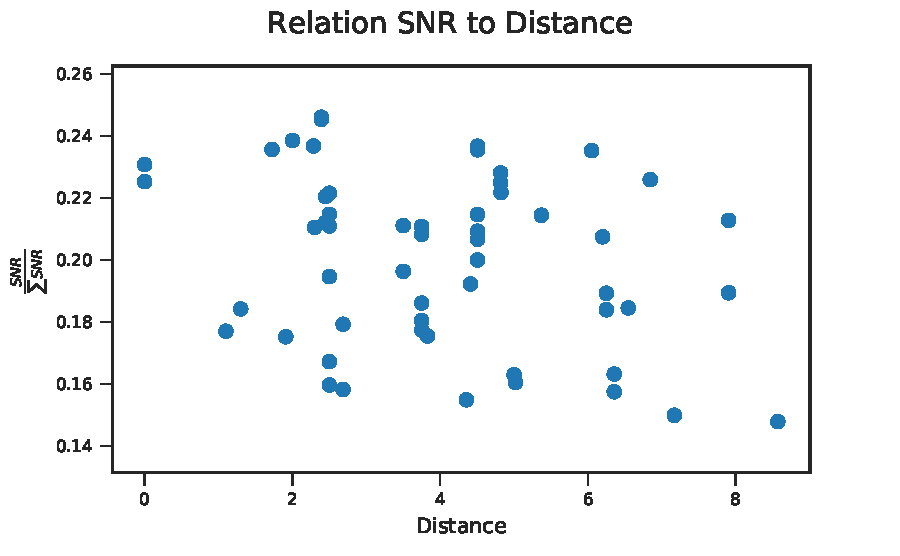
\includegraphics[]{figures/evaluation/snr_scatter}
	\caption{Visualization of relation between SNR and distance.}
	\label{fig:04_snrDistance}
\end{figure}
% -------------------------------------------------------------

Due to the result, further analysis on the \ac{SNR} values
on individual robots is done for evaluation of the microphones' validity.
For this purpose, a signal is played back digitally from fixed distance
and constant volume with different angles.
The main purpose of this measurement is to ensure that the lone channels
are not biased.
14 measurements of a 3\si{\kilo\hertz} sine signal
with are distance of 0.73\si{m} are done but no tendency is detectable.
Further evaluation is done by determining the channel with the maximum
\ac{SNR} of one measurement.
It is expected that the nearest channel to the sound source has maximum \ac{SNR}.
At 85,71\si{\percent} of the cases this assertion could be evidenced.
From this, it can be said that the general recordings of the microphones
are neither biased nor falsified.

The same procedure is done with the real whistle recordings of the
measurement in \ref{subsec:04_labMeasurements}.
Using these measurements, only 54,55\si{\percent} of the maximum \acp{SNR}
match with the expected channels.
Consequentially, one must assume that the environmental circumstances
like multi-path propagation and reflection have large influence
on the signal data.
Thus, neither for a single robot direction result nor for the team filter
the \ac{SNR} can be utilized.

\subsection{PSNR}
\label{subsec:04_psnr}

As referred in \cref{sec:02_gcc}, the main characteristic of the \ac{GCC-PHAT}
algorithm is the emerging sharp peak.
In conclusion, one can assume that the lack of a sharp peak indicates
a less valid delay result of the \ac{GCC}.

\subsubsection*{Informative Value}

This statement is examined by comparing the \ac{PSNR} value
to the error of the direction angle resulting from the \ac{GCC-PHAT} delay.
% Two cases of errors are taken into consideration.
In the following, the \ac{PSNR} is recorded as high if it exceeds 17,5 whereat the
\ac{PSNR} value ranges from 10,1 to 28,8 for measurements in
\cref{subsec:04_labMeasurements}.

Firstly, it is looked at each channel pair by determining the
error between true direction and the most suited direction candidate emerging
from the \ac{GCC} delay.
The results are split by the \ac{PSNR} value.
If the \ac{PSNR} of the \ac{GCC} is greater than the threshold of 17,5,
the \ac{RMSE} of its result is grouped to the errors with high \ac{PSNR}.
Elsewise it pertains to the errors with low \ac{PSNR}.
This valuation is done with the measurements of \cref{subsec:04_labMeasurements}
and manually set start indexes.
Having 76 correlations assessed with low \ac{PSNR}, the \ac{RMSE} of this group
is 35,77\si{\degree}.
Compared to this, the \ac{RMSE} of the remaining 144 measurements
is 15,86\si{\degree} only.

To see the impact on a complete robot result, the same is done
with the final angular errors of single robots results.
Here, the \ac{RMSE} of the lower \ac{PSNR} case results in 25,36\si{\degree}
whereat the error of the other case is 14,41\si{\degree}.
From this, one can identify the \ac{PSNR} as valid enriching information.

\subsubsection*{Frame Selection}

Another perspective is to include the PSNR information into the single
robot whistle direction determination.
In \cref{fig:04_psnr2FrameShift}, the frame to investigate is
shifted before and after the signal start index.
Here, the same measurement as in \cref{sec:04_tdoaSingle} is used where
the robot was positioned at the center point
while the whistle is blown at -33,7\si{\degree} with 4,5\si{\meter}
distance.
The frame size of the \ac{GCC} is set to 256 samples and the shift
was set to a quarter of the frame size.
Samples of the rear left channel are plotted for better understanding
in the upper graph of \cref{fig:04_psnr2FrameShift}.
The second graph shows the \ac{RMSE} of the robot direction result
over the frame shifts.
For the lower graph, the mean over the \acp{PSNR} of all channels
is presented.
One sees, how the error is low with high \ac{PSNR} what confirms
the previous statement in this section.
For shifts smaller than -2, the signal is not represented in the
frames yet what explains the high error.
An important notice is that the result changes with proceeding
frames what indicates that the implemented \ac{GCC-PHAT} method is
not suitable for arbitrary frames.
% Without additional information about the rough direction,
% ambiguity exists due to periodicity of the signal.
% Due to the inconclusive result of the \ac{SNR} in \cref{subsec:04_snr}
% one decides not to take the signal magnitude as such information
% into account.
% Thus, the decisive role of the start of the signal is underlined again.
% -------------------------------------------------------------
\begin{figure}[ht]
	\centering
	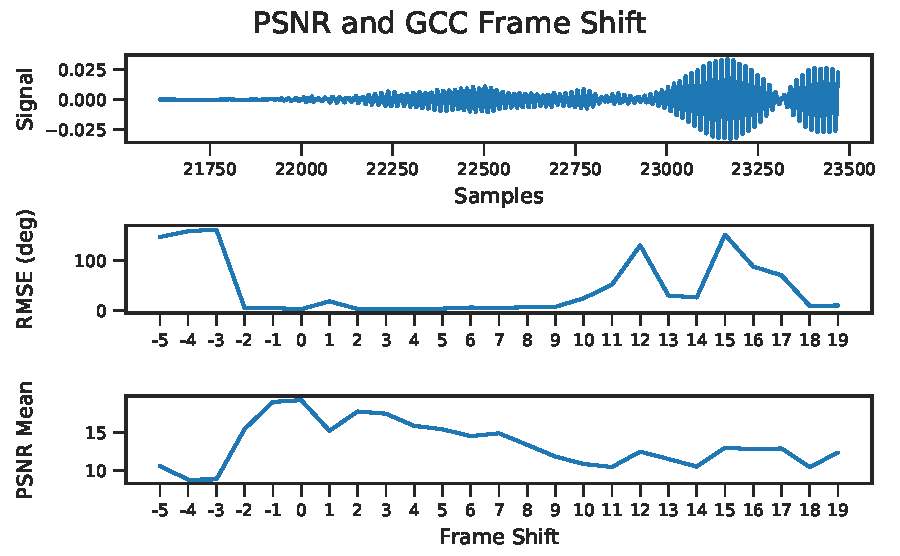
\includegraphics[]{figures/evaluation/gcc_frame_shift}
	\caption{
		Relation between \ac{PSNR}
		and selection of the frame in time. Signal data
		of the rear left channel is plotted in the upper window.
		In this measurement, the whistle is positioned at right front
		of the robot.
	}
	\label{fig:04_psnr2FrameShift}
\end{figure}
% -------------------------------------------------------------


